\section{Project Setup}
The following components were present in the lab:

\begin{itemize}
    \item Model Car: The model car has three servos for the brakes, one servo for steering and an engine for acceleration. All of these components are controlled via a servo controller board.
   
    \item Servo Controller Board: The servo controller board is a \textit{pololu maestro servo controller board} which is attached to a Raspberry Pi via a usb-to-uart bridge.
   
    \item Raspberry Pi: The Raspberry Pi is responsible for sending control commands to the servo controller board. It receives its input data from a PandaBoard via a mqtt topic to which it is subscribed. The Raspberry Pi runs Genode with Fiasco.OC.
   
    \item PandaBoard: Besides the Raspberry Pi, the PandaBoard is the second ECU in the model car. It also runs Genode with Fiasco.OC. The task is to receive data from a simulation, transform the data into concrete servo values and send them via mqtt to the Raspberry Pi.
\end{itemize}

An image of the model car is shown in figure \ref{fig:model}. The servos can be seen in box a. Box b shows the Raspberry Pi. The PandaBoard is placed on top of the car and can be seen in box c. The servo controller board is placed behind the Raspberry Pi which can not be seen in the image. \\

\begin{figure}[h]
       \centering
       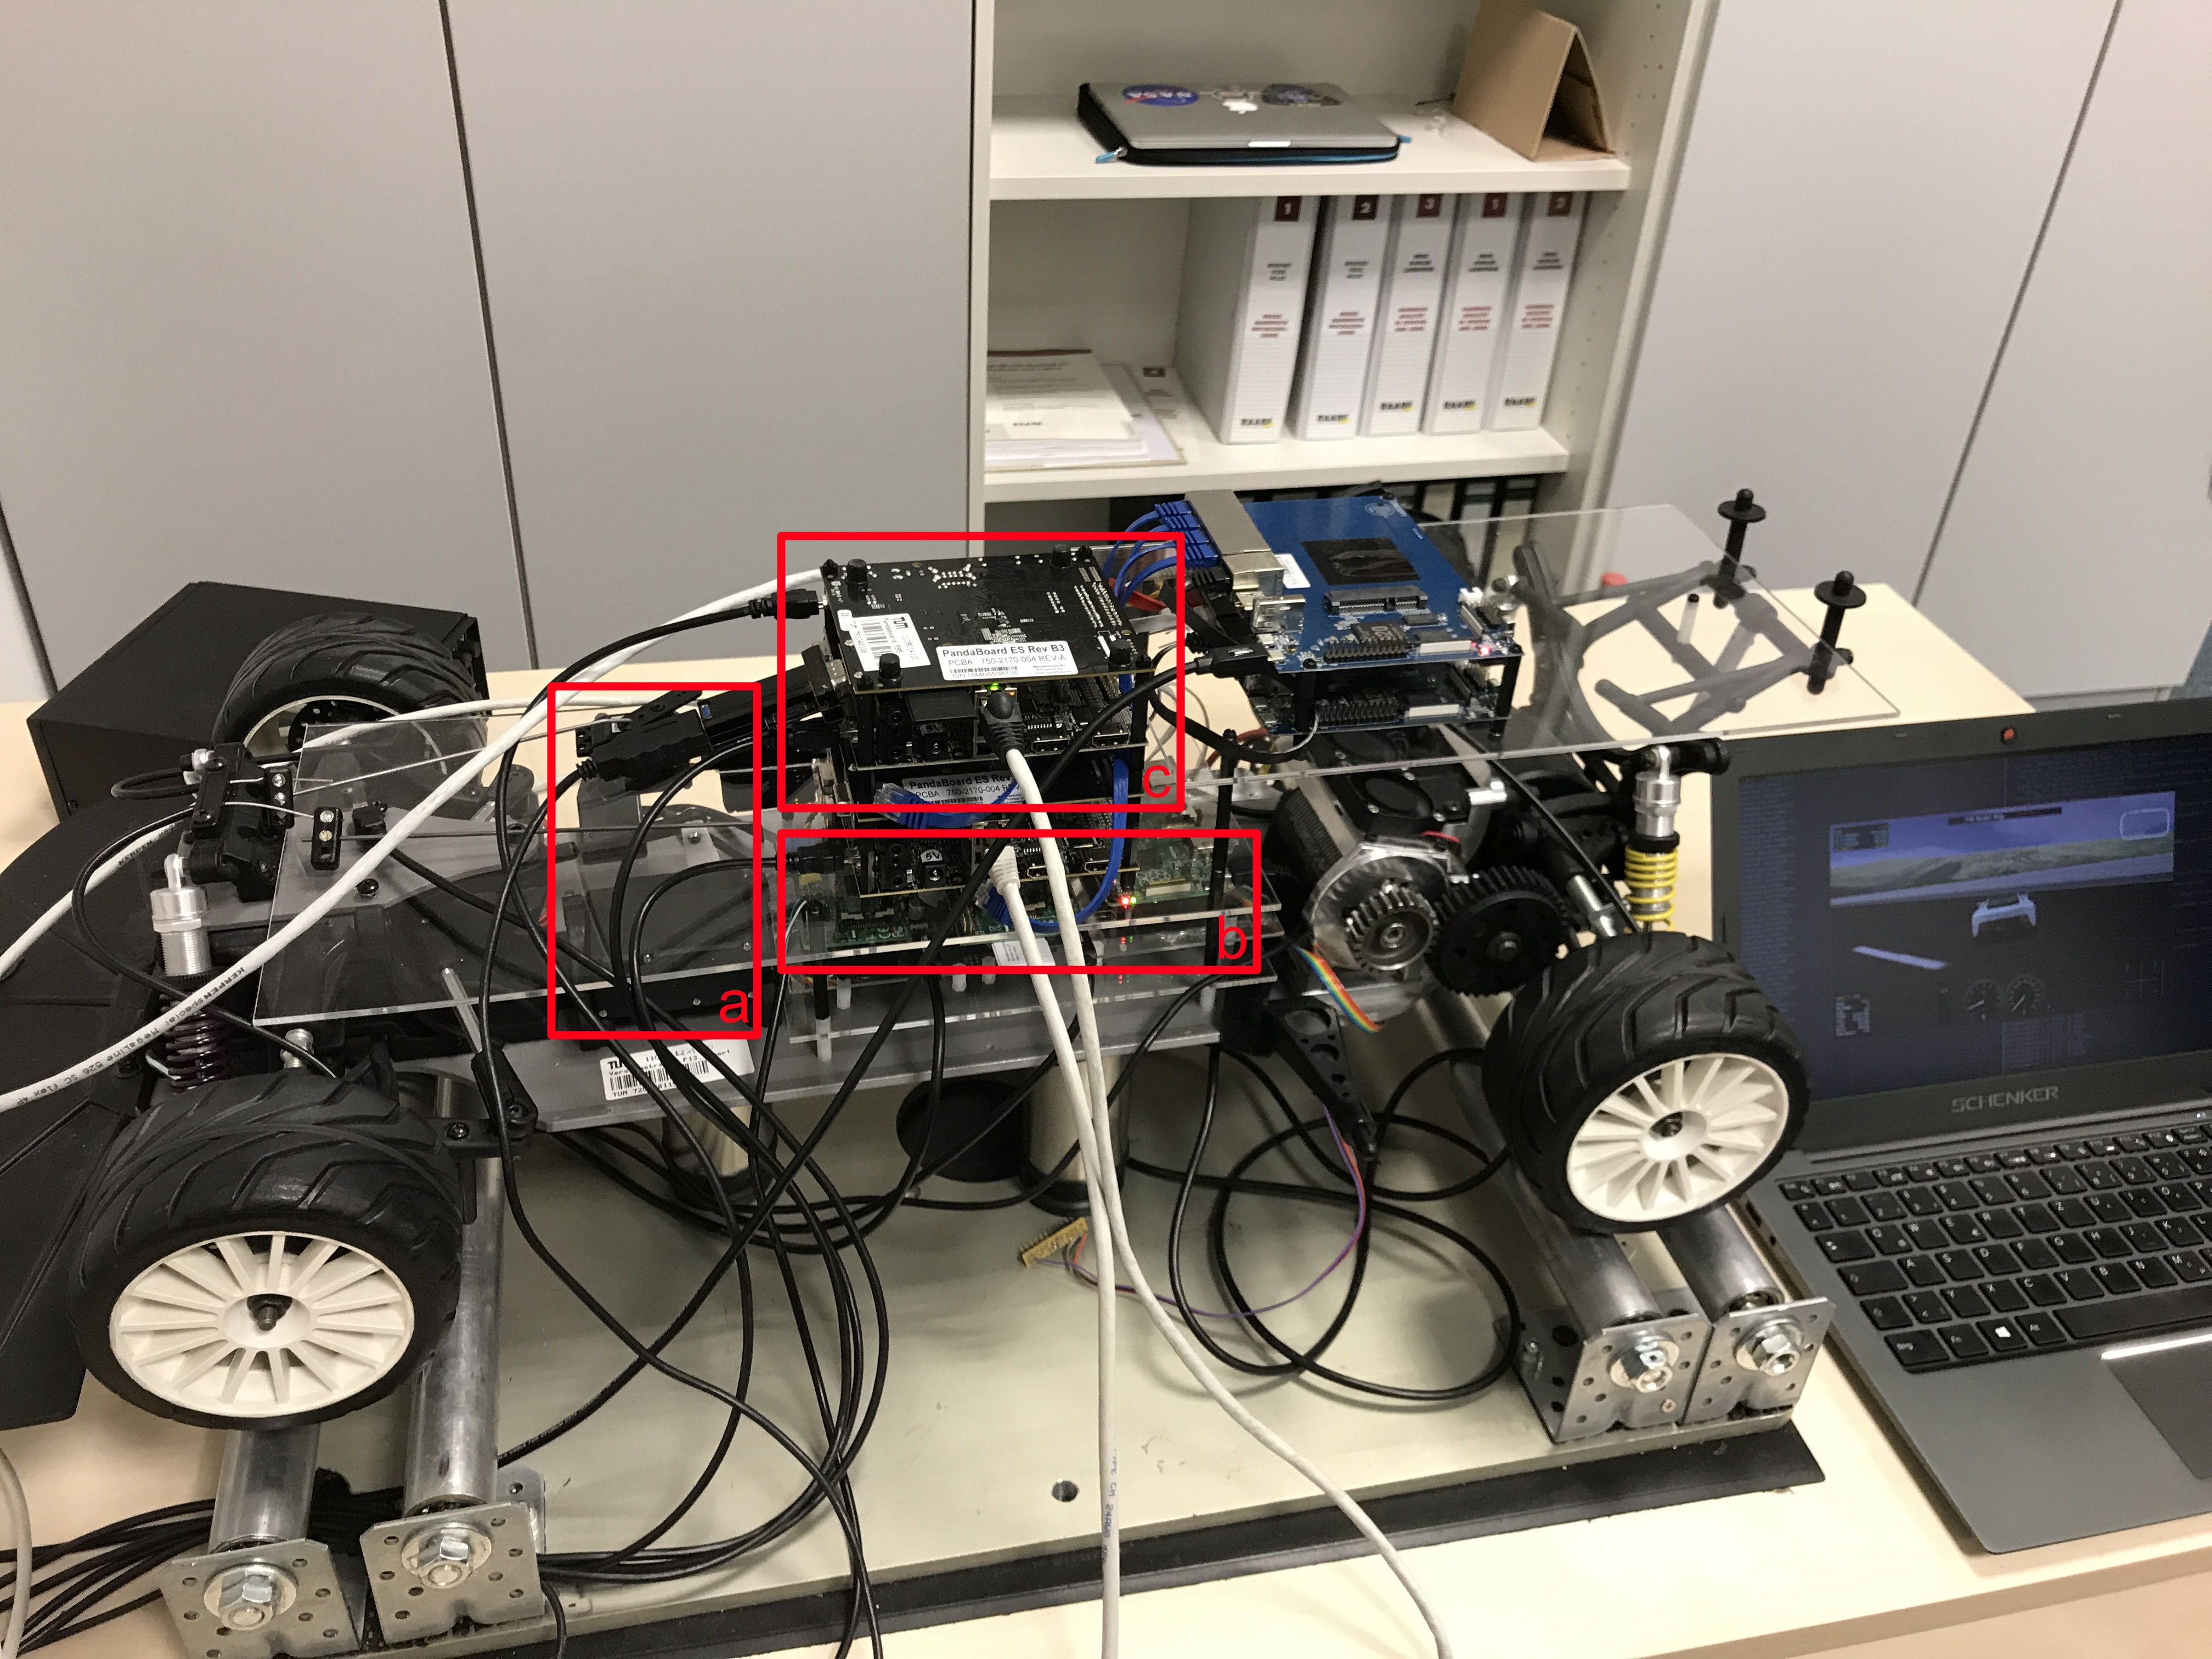
\includegraphics[trim={0 5cm 0 30cm},clip,width=1.0\linewidth]{images/model}
       \caption{Model Car}
       \label{fig:model}
\end{figure}

\newpage

%%%%%%%%%%%%%%%%%%%%%%%%%%%%%%%%%%%%%%%%%%%%%%%%%%%%%%%%%%%%
\section{Source Code Structure}

\dirtree{%
.1 car\_project.
.2 run.
.2 include.
.3 controller\_session.
.3 servo\_session.
.2 src.
.3 mqtt.
.3 rpi\_component.
.4 rpi.
.4 servo.
.3 panda\_component.
.4 panda.
.4 controller.
.2 old.
.3 linux.
.3 pololu.
}


\paragraph{run}
In the run folder the run files for the ecu (\texttt{car\_panda.run}) and the servo controller (\texttt{car\_rpi.run}) are placed.
These are responsible for defining the project build components and the boot modules. Additionally, they contain the configuration for the started modules.

\paragraph{include}
In the include directory the header files for the servo and the controller component are split up into their respective folders.

\paragraph{include/servo\_session}
Contains the interface for the \texttt{servo\_session} component described in section~\ref{sec:comp-servo}.

\paragraph{include/controller\_session}
Contains the interface for the \texttt{controller\_session} component described in section~\ref{sec:comp-controller}.

\paragraph{src}
In the source (\texttt{src}) directory all source files used can be found.
Each of the two targets is further split up into its main component and a secondary component including each a target.mk for the build process and the actual \CC-source file.

\paragraph{src/mqtt}
In the subdirectory mqtt is a class that implements the mosquitto interface, which is used in the panda and the rpi targets.

\paragraph{src/rpi\_component}
The \texttt{rpi\_component} contains the programs that run on the Raspberry Pi described by the \texttt{car\_rpi.run} runfile.

\paragraph{src/rpi\_component/rpi}
The rpi program is responsible for handling the commands received from the mqtt server and forwarding them to the servo program

\paragraph{src/rpi\_component/servo}
The servo program controls the servos by sending commands over the serial connection which connects the Raspberry Pi and the pololu servo controller board.

\paragraph{src/panda\_component}

\paragraph{src/panda\_component/panda}

\paragraph{src/panda\_component/controller}

\paragraph{old}
The old folder contains programs and scripts used for development.

\paragraph{old/linux}
An implementation of the rpi and panda components as linux user programs can be found in the \texttt{linux} folder.
These were used for development during the first phase of the project when the rpi genode image was available yet.

\paragraph{old/pololu}


%%%%%%%%%%%%%%%%%%%%%%%%%%%%%%%%%%%%%%%%%%%%%%%%%%%%%%%%%%%%
\section{Application Programming Interfaces}

%%%%%%%%%%%%%%%%%%%%%%%%%%%%%%%%%%%%%%%%%%%%%%%%%%%%%%%%%%%%
\subsection{Mqtt component}
We use mqtt for both, the communication between the simulation and the PandaBoard and the communication between the PandaBoard and the Raspberry Pi.

\subsubsection{car-control}
This is the topic name of the mqtt topic to which the PandaBoard is subscribed to. Commands to this topic are sent from the simulation. All commands need to have the following format: \\

\textbf{Format:} (command,value) \\
Command describes the type of request, i.e. braking, steering or acceleration. Value describes the strength of the command. All possible commands and values are listed in table \ref{tab:car-control}. \\

\textbf{Example:} (1,0.5) \\
This is a brake request with half braking force \\

\begin{figure}[h]
    \centering
    \begin{tabular}{c | c | c}
        \textbf{Command} & \textbf{Value Range} & \textbf{Meaning} \\ \hline
        0   &   [ -1.0 ; 1.0 ]    & Steering \\
        1   &   [ 0 ; 1.0 ]       & Brake \\ 
        2   &   [ 0 ; 1.0 ]       & Acceleration \\ 
    \end{tabular}
    \caption{Allowed values for the car-control topic}
    \label{tab:car-control}
\end{figure}


\subsubsection{car-servo}
This is the topic name of the mqtt topic to which the Raspberry Pi is subscribed to. Commands to this topic are sent from the PandaBoard. All commands need to have the following format: \\ 

\textbf{Format:} (channel,value) \\
Channel is a number ranging from 0 to 11 and describes the channel number on the servo controller board. The braking servos are connected to channels 0, 1 and 2, whereas the steering servo is connected to channel 6. With the pololu maestro servo controller board it is not possible to control the engine. Values are pwm signals ranging from 4500 to 7500. The neutral value for the servo is 6000. \\

\textbf{Example:} (0,7500) \\
This command sends a pwm signal with value 7000 to channel 0. This means that the brake connected to channel 0 gets activated with full force. 

%%%%%%%%%%%%%%%%%%%%%%%%%%%%%%%%%%%%%%%%%%%%%%%%%%%%%%%%%%%%
\subsection{Components interface}
\label{sec:comp}


\subsubsection{Servo component}
\label{sec:comp-servo}

The servo component provides five methods. All methods return -1 if an error occurred and else 0 or the requested value.
\begin{itemize}
\item The function \textbf{setTarget} receives a channel, where the servo is connected and the target position.
\item The function \textbf{setSpeed} receives a channel, where the servo is connected and the maximum speed of the servo, where 0 means unlimited.
\item The function \textbf{setAcceleration} receives a channel, where the servo is connected and the maximum acceleration of the servo, where 0 means unlimited.
\item The function \textbf{getPosition} receives a channel, where the servo is connected and returns its current position.
\item The function \textbf{getMovingState} returns 0 if no servo is moving else 1.
\end{itemize}

\begin{lstlisting}[language=c, frame=single, basicstyle=\footnotesize, caption=Genode interface for servo component]
GENODE_RPC(Rpc_setTarget, int, setTarget, unsigned char, unsigned short);
GENODE_RPC(Rpc_setSpeed, int, setSpeed, unsigned char, unsigned short);
GENODE_RPC(Rpc_setAcceleration, int, setAcceleration, unsigned char, 
						      unsigned short);
GENODE_RPC(Rpc_getPosition, int, getPosition, unsigned char);
GENODE_RPC(Rpc_getMovingState, int, getMovingState);
\end{lstlisting}

\subsubsection{Controller component}
\label{sec:comp-controller}

The controller component provides two methods each expecting a double as input and returning an integer value.
\begin{itemize}
\item The function \textbf{transform\_steer} transforms a steering angle between -1 and 1, where -1 is completely right, and returns the corresponding pwm value in quarter microseconds for the servo.
\item The function \textbf{transform\_brake} transforms a braking value between 0 and 1, where 1 means fully applied, and returns the corresponding pwm value in quarter microseconds for the servo.
\end{itemize}

\begin{lstlisting}[language=c, frame=single, basicstyle=\footnotesize, caption=Genode interface for controller component]
GENODE_RPC(Rpc_transform_steer, int, transform_steer, double);
GENODE_RPC(Rpc_transform_brake, int, transform_brake, double);
\end{lstlisting}